\begin{landscape}

\section{Diseño Lógico de la Topología}

\begin{figure}[H]
\centering
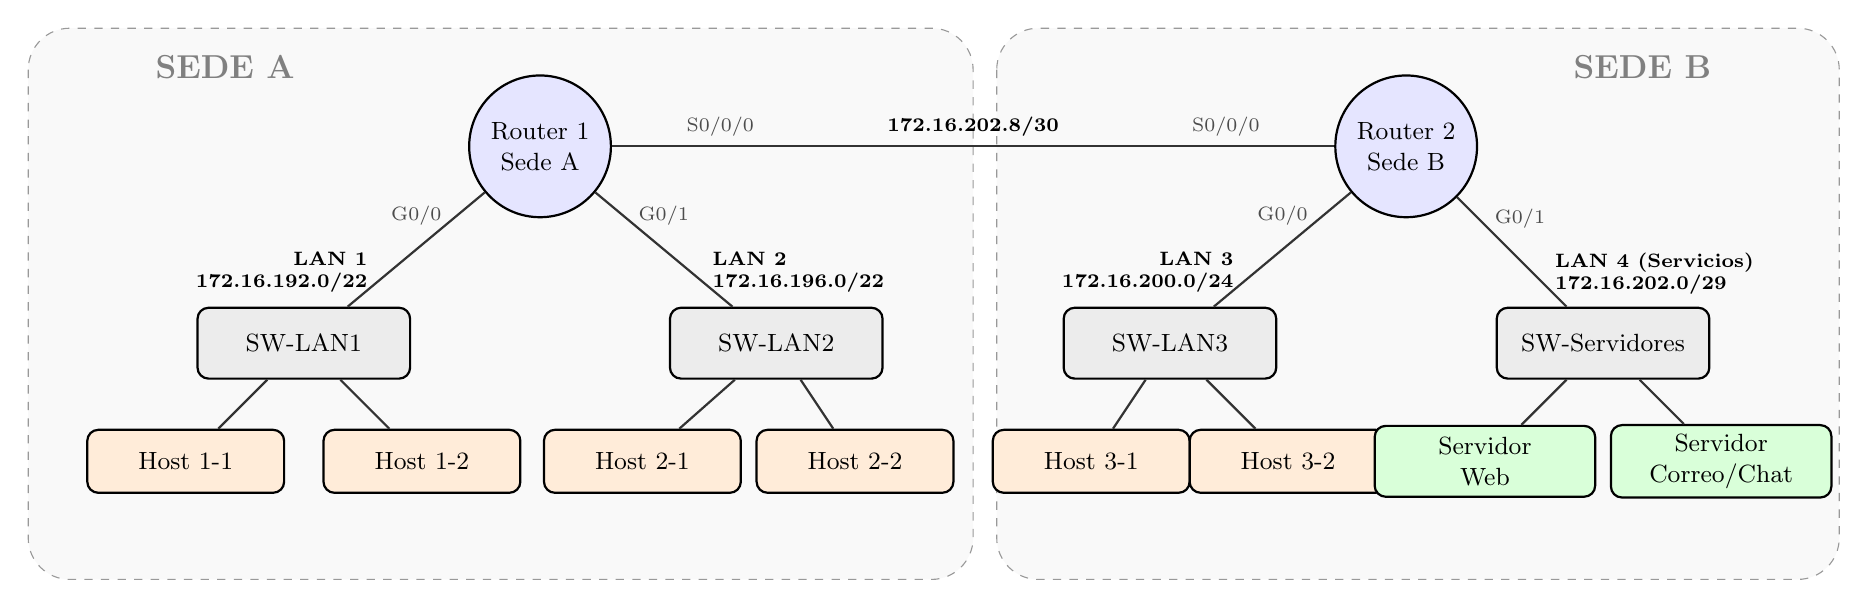
\begin{tikzpicture}[
    font=\small,
    % Cambiamos los routers a forma circular (estándar)
    router/.style={draw, circle, thick, minimum size=1.8cm, align=center, fill=blue!10},
    switch/.style={draw, rounded corners, thick, minimum width=2.7cm, minimum height=0.9cm, align=center, fill=gray!15},
    server/.style={draw, rounded corners, thick, minimum width=2.8cm, minimum height=0.9cm, align=center, fill=green!15},
    client/.style={draw, rounded corners, thick, minimum width=2.5cm, minimum height=0.8cm, align=center, fill=orange!15},
    % Las conexiones de red no llevan flechas direccionales
    link/.style={thick, draw=black!80},
    % Estilos para etiquetas de interfaces y subredes
    intf/.style={font=\scriptsize, text=black!70},
    subnet/.style={font=\scriptsize\bfseries, text=black}
]

% --- Fondos para agrupar las sedes ---
\draw[dashed, draw=gray!80, fill=gray!5, rounded corners=15pt] (-6.5, 1.5) rectangle (5.5, -5.5);
\node[font=\large\bfseries, text=gray] at (-4, 1) {SEDE A};

\draw[dashed, draw=gray!80, fill=gray!5, rounded corners=15pt] (5.8, 1.5) rectangle (16.5, -5.5);
\node[font=\large\bfseries, text=gray] at (14, 1) {SEDE B};

% --- Routers ---
\node[router] (r1) at (0,0) {Router 1\\Sede A};
\node[router] (r2) at (11,0) {Router 2\\Sede B};

% --- Enlace WAN ---
\draw[link] (r1) -- node[above, subnet] {172.16.202.8/30} node[pos=0.15, intf, above] {S0/0/0} node[pos=0.85, intf, above] {S0/0/0} (r2);

% --- SEDE A - LAN 1 ---
\node[switch] (sw1) at (-3,-2.5) {SW-LAN1};
\node[client] (c1a) at (-4.5,-4) {Host 1-1};
\node[client] (c1b) at (-1.5,-4) {Host 1-2};

\draw[link] (r1) -- node[pos=0.2, intf, left=2pt] {G0/0} node[pos=0.7, subnet, left=4pt, align=right] {LAN 1\\172.16.192.0/22} (sw1);
\draw[link] (sw1) -- (c1a);
\draw[link] (sw1) -- (c1b);

% --- SEDE A - LAN 2 ---
\node[switch] (sw2) at (3,-2.5) {SW-LAN2}; 
\node[client] (c2a) at (1.3,-4) {Host 2-1};
\node[client] (c2b) at (4,-4) {Host 2-2};

\draw[link] (r1) -- node[pos=0.2, intf, right=2pt] {G0/1} node[pos=0.7, subnet, right=4pt, align=left] {LAN 2\\172.16.196.0/22} (sw2);
\draw[link] (sw2) -- (c2a);
\draw[link] (sw2) -- (c2b);

% --- SEDE B - LAN 3 ---
\node[switch] (sw3) at (8,-2.5) {SW-LAN3};
\node[client] (c3a) at (7,-4) {Host 3-1};
\node[client] (c3b) at (9.5,-4) {Host 3-2};

\draw[link] (r2) -- node[pos=0.2, intf, left=2pt] {G0/0} node[pos=0.7, subnet, left=4pt, align=right] {LAN 3\\172.16.200.0/24} (sw3);
\draw[link] (sw3) -- (c3a);
\draw[link] (sw3) -- (c3b);

% --- SEDE B - LAN 4 ---
\node[switch] (sw4) at (13.5,-2.5) {SW-Servidores};
\node[server] (srv1) at (12,-4) {Servidor\\Web};
\node[server] (srv2) at (15,-4) {Servidor\\Correo/Chat};

\draw[link] (r2) -- node[pos=0.2, intf, right=2pt] {G0/1} node[pos=0.7, subnet, right=4pt, align=left] {LAN 4 (Servicios)\\172.16.202.0/29} (sw4);
\draw[link] (sw4) -- (srv1);
\draw[link] (sw4) -- (srv2);

\end{tikzpicture}
\caption{Topología lógica con asignación de interfaces y subredes IPv4}
\label{fig:topologia}
\end{figure}

\end{landscape}